\begin{figure}[t]
\centering
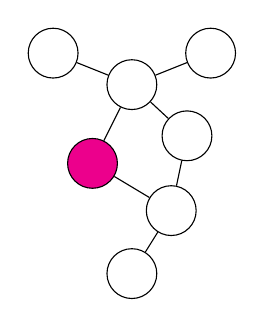
\begin{tikzpicture}
  \tikzstyle{node}=[circle,draw, minimum width=18pt, inner sep=0pt, fill=white]
  \tikzstyle{root}=[fill=magenta]

  \node[node, root] (1) at (0,    0)    {};
  \node[node]       (2) at (0.5,  1)    {};
  \node[node]       (3) at (1,    -0.6) {};
  \node[node]       (4) at (1.2,  0.35) {};
  \node[node]       (5) at (1.5,  1.4)  {};
  \node[node]       (6) at (-0.5, 1.4)  {};
  \node[node]       (7) at (0.5,  -1.4) {};

  \path (1) edge (2);
  \path (1) edge (3);
  \path (2) edge (4);
  \path (2) edge (5);
  \path (2) edge (6);
  \path (3) edge (4);
  \path (3) edge (7);
\end{tikzpicture}
\caption[Normalisierung für Graphen im zweidimensionalen Raum]{}
\label{fig:normalisierung_erweitert}
\end{figure}
